\subsection{MOT}
While the dissipative force slows atoms down, it does not provide a spatial confinement. In cold atom experiments, to achieve quantum degeneracy, the density of phase needs to be high enough which requires a high spatial density. In \cite{raab1987trapping},scientists proposed to combine optical molasses with a magnetic field gradient, it cools and traps atoms at the same time.

\begin{figure}[htbp]
    \centering
    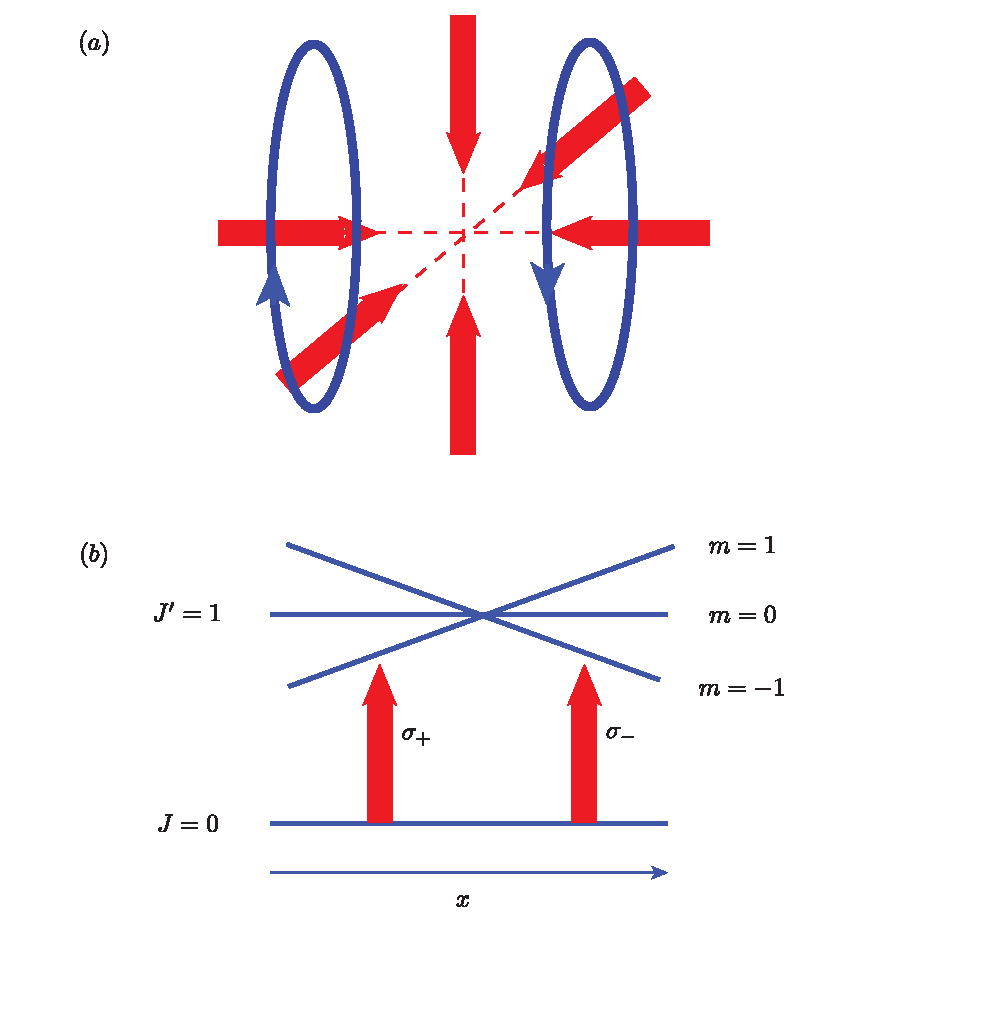
\includegraphics[width=\textwidth]{Chapter2_secs/MOT.pdf}
    \caption{MOT. (a) A sketch of MOT, three pairs of counter propagating laser beams are combined with a pair of anti-Helmholtz coil. (b)Energy levels of $\ket{J=0}$ and $\ket{J=1}$, coupled by $\sigma_+$ and $\sigma_-$ polarized beams. }
    \label{fig:MOT}
\end{figure}

Fig.~(\ref{fig:MOT})(a) shows the sketch of a MOT. It combines 3D optical molasses with a pair of anti-Helmholtz coil. The magnetic field generated by the anti-Helmholtz coil is in the form
\begin{equation}
    \Vec{B}(\Vec{r}) = b(x\textbf{e}_x + y\textbf{e}_y - 2z\textbf{e}_z)
\end{equation}
The energy levels of $\ket{J=0}$ and $\ket{J=1}$ states are drawn in Fig.~(\ref{fig:MOT})(b) as a function of position due to Zeeman shift. The detuning of $\sigma_+$ and $\sigma_-$ are thus a function of position \cite{metcalf2007laser}. 
\begin{equation}
    \delta_\pm (\Vec{v},\Vec{r}) = \delta_0 \mp \Vec{k}\cdot \Vec{v} \pm \mu'\cdot \Vec{B}(\Vec{r})/\hbar
\end{equation}
Here $\mu' = (g_{J'} m_{J'} - g_{J} m_{J})\mu_B$.

Intuitively, as atoms move to the left of the trap center, the $\sigma_+$ beam is closer to resonance with the transition between $\ket{m_J=0}$ and $\ket{m_J=1}$. The optical pumping effect from the $\sigma_+$ beam is stronger and the overall force points to the right. As atoms move to the right, it is the other way around, the $sigma_-$ beam is closer to resonance and has stronger optical pumping effect. Thus, MOT provides a spatial restoring force. Together with the dissipative force, the total force is
\begin{equation}
    \Vec{F} = -\beta \Vec{v} - \kappa \Vec{r}.    
\end{equation}
$\kappa = \mu'\beta b /\hbar k$.
